Measurements of the activity of additional jets (jets not coming from the decay of top quarks)
have been made by ATLAS~\cite{gapfraction,hdamp,ljets} and CMS\cite{Chatrchyan:2014gma} using
pp data with $\sqrt{s}=7~\TeV$.  Comparison of the measured distributions with the predictions of Monte Carlo (MC) generators
indicate that some state-of-the-art generators (e.g. \textsc{MC@NLO}) have a difficult time in reproducing the data,
while for others  agreement with data can be improved with appropriate
choice of generator parameters.  For example, in \textsc{Powheg+Pythia} adding a damping
function that limits the resummation of higher-order effects incorportated into  the Sudakov form factor improves
the agreement between data and MC~\cite{hdamp} at 7~TeV.  

The range of predictions observed in standard MC generators for
8~\TeV\ $pp$ interactions is shown in 
Figure~\ref{fig:introtjets}. The fiducial definition of these extra jets is provided in Chapter~\ref{ch:extrajets}.  
Differences in rate as large as 40\%\  are seen for
jet multiplicities $\ge 5$.  Differences up to 20\%\ for the leading
jet and up to 40\%\ for the subleading jet are seen at high jet transverse
momentum.  
\begin{figure}
\centering
\begin{subfigure}[]{0.45\textwidth}
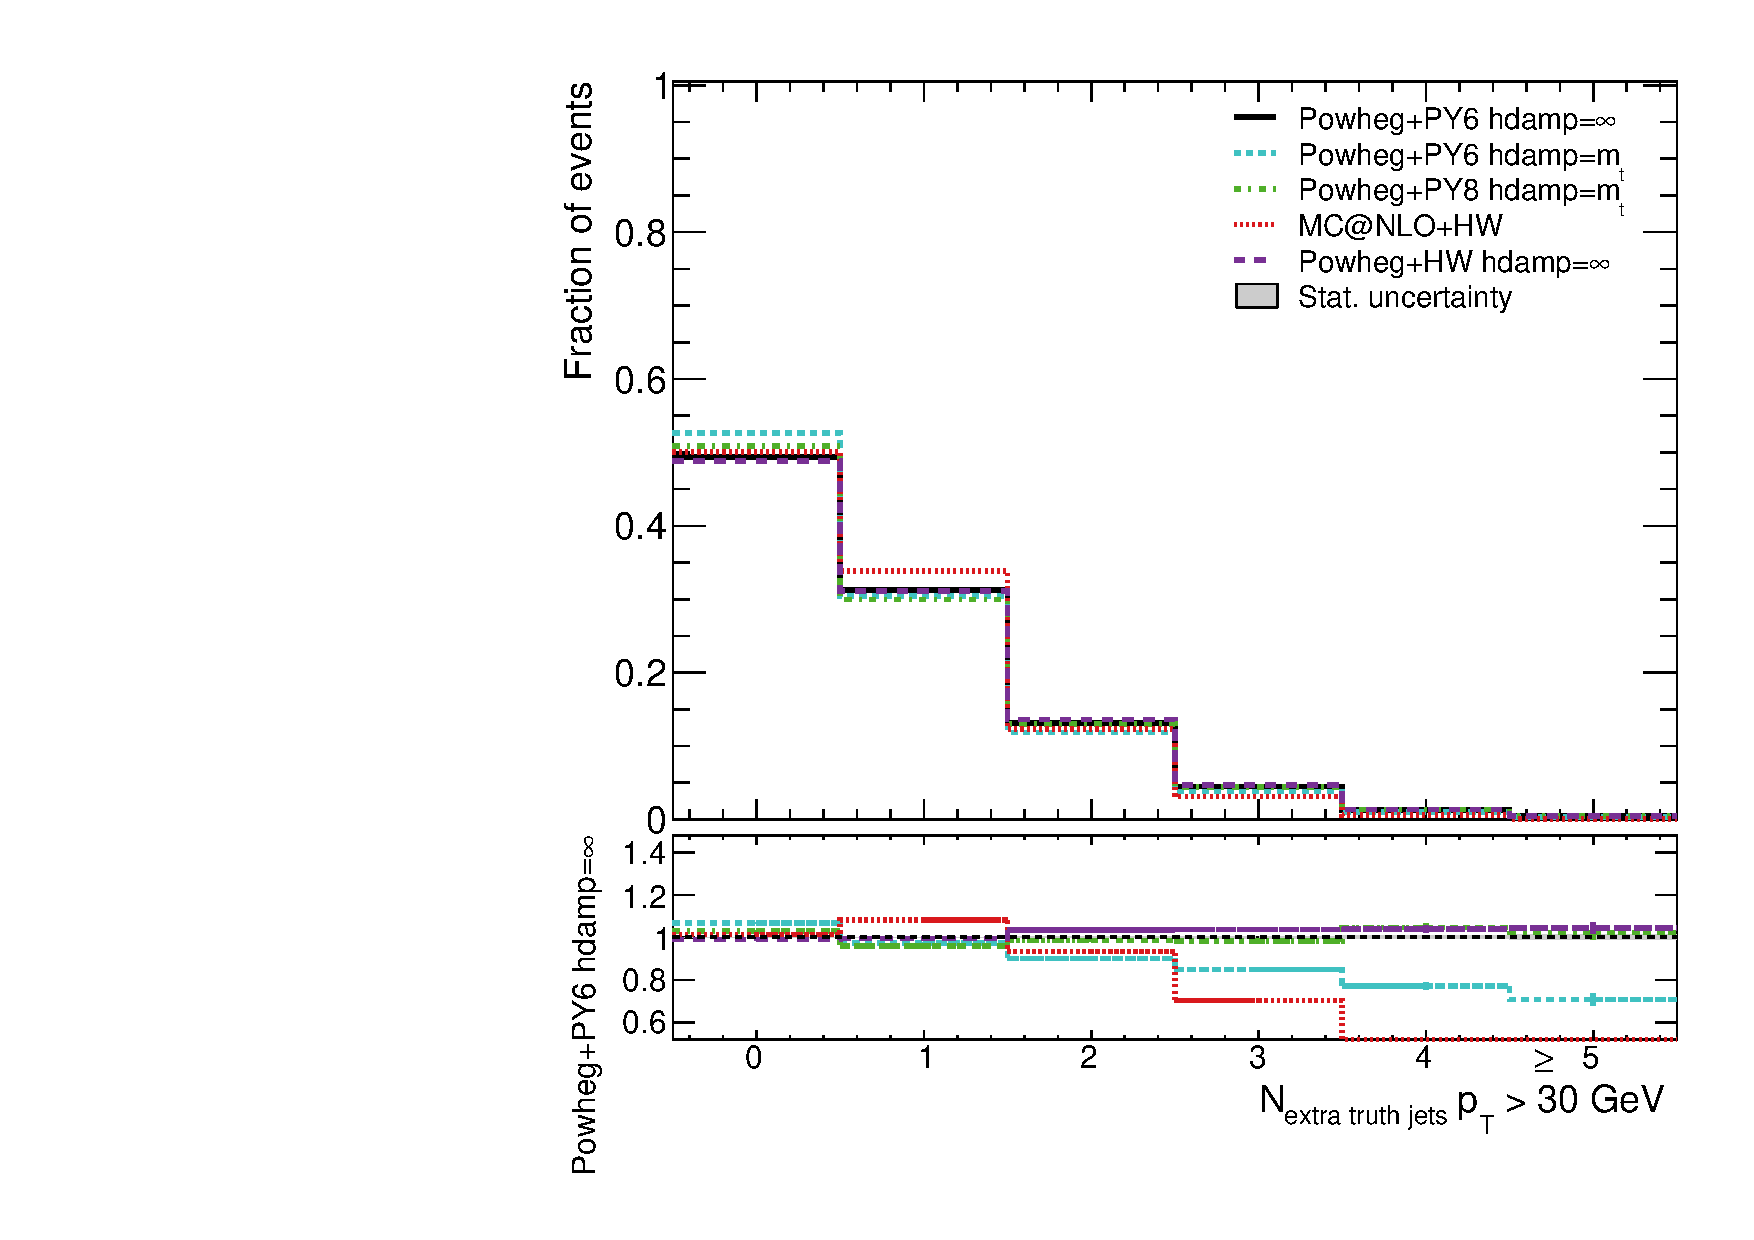
\includegraphics[width=\textwidth]{fig/MCComp/NLO/NTruthExtraJets30.pdf}
\end{subfigure}
~
\begin{subfigure}[]{0.45\textwidth}
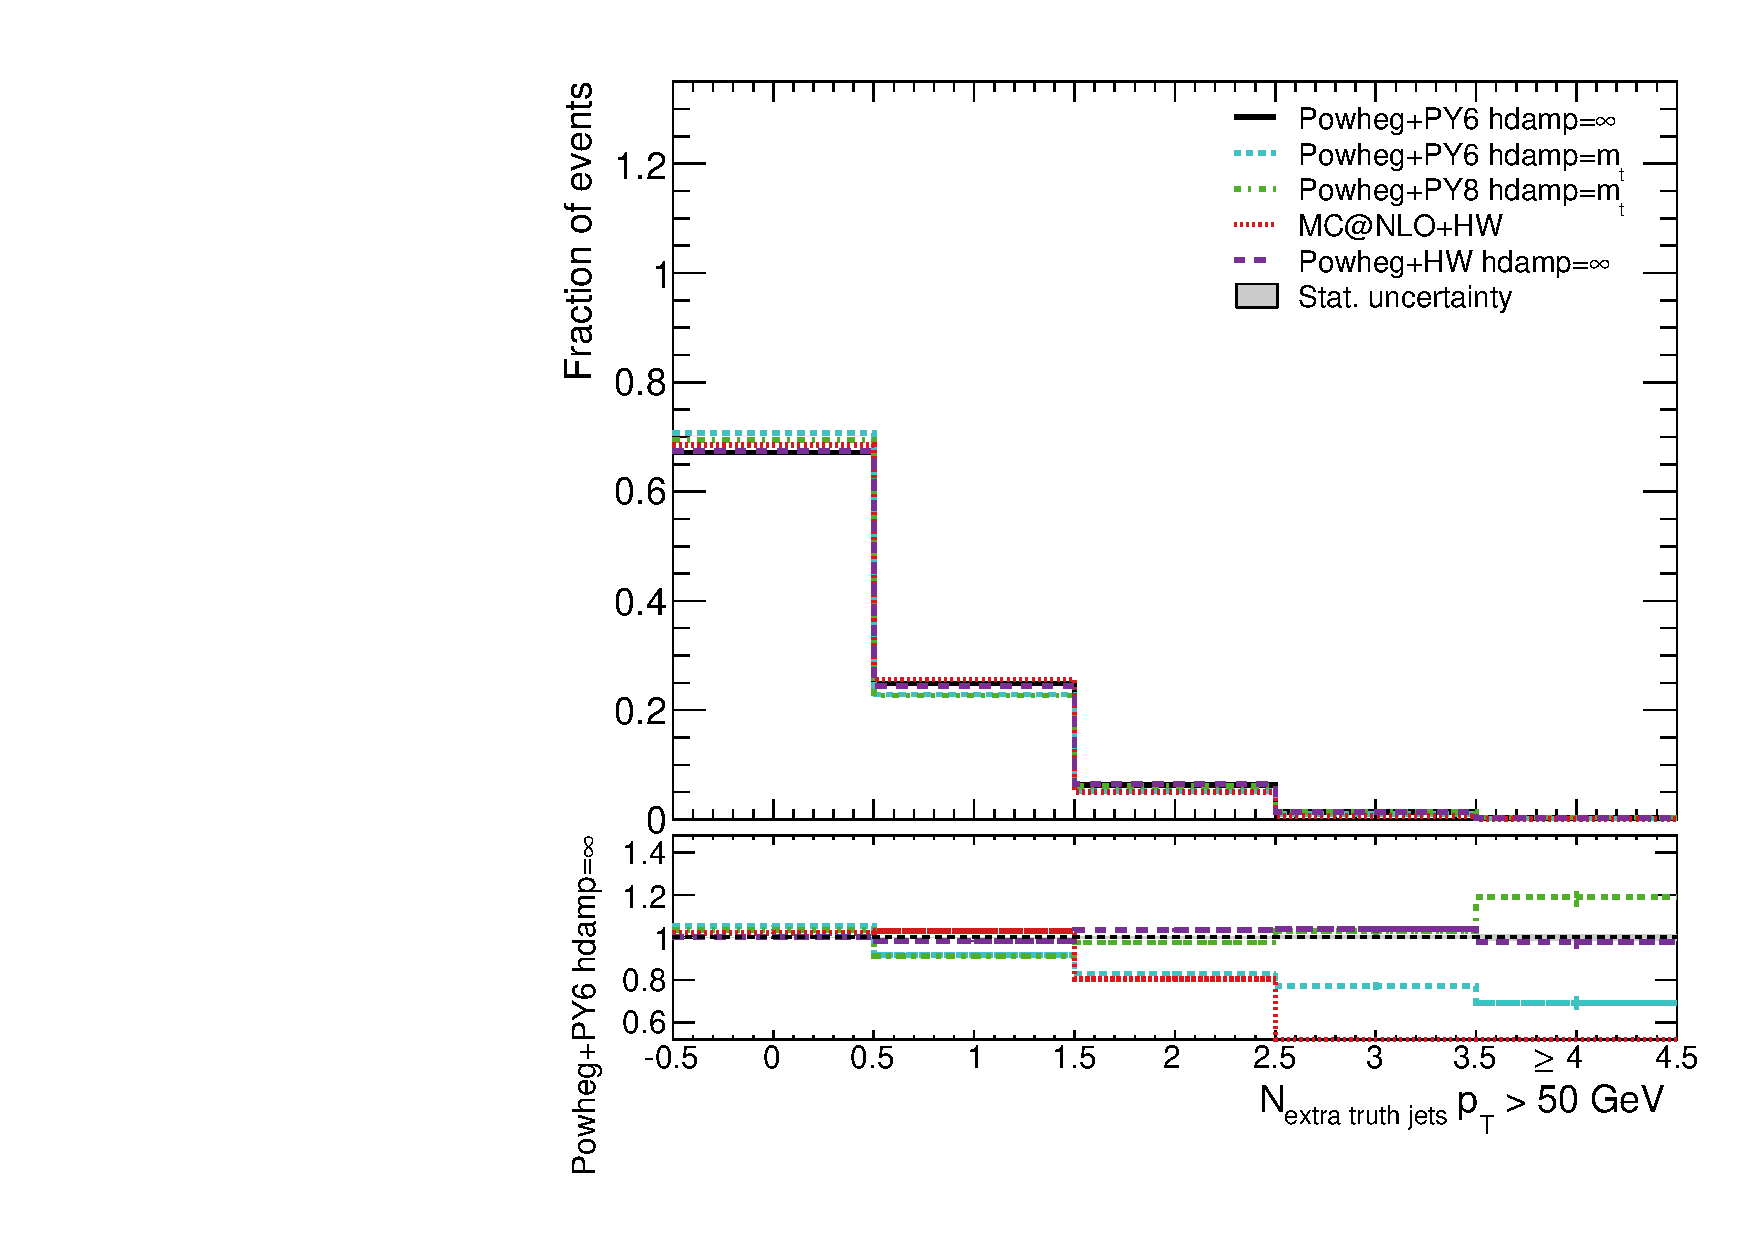
\includegraphics[width=\textwidth]{fig/MCComp/NLO/NTruthExtraJets50.pdf}
\end{subfigure} \\
\begin{subfigure}[]{0.45\textwidth}
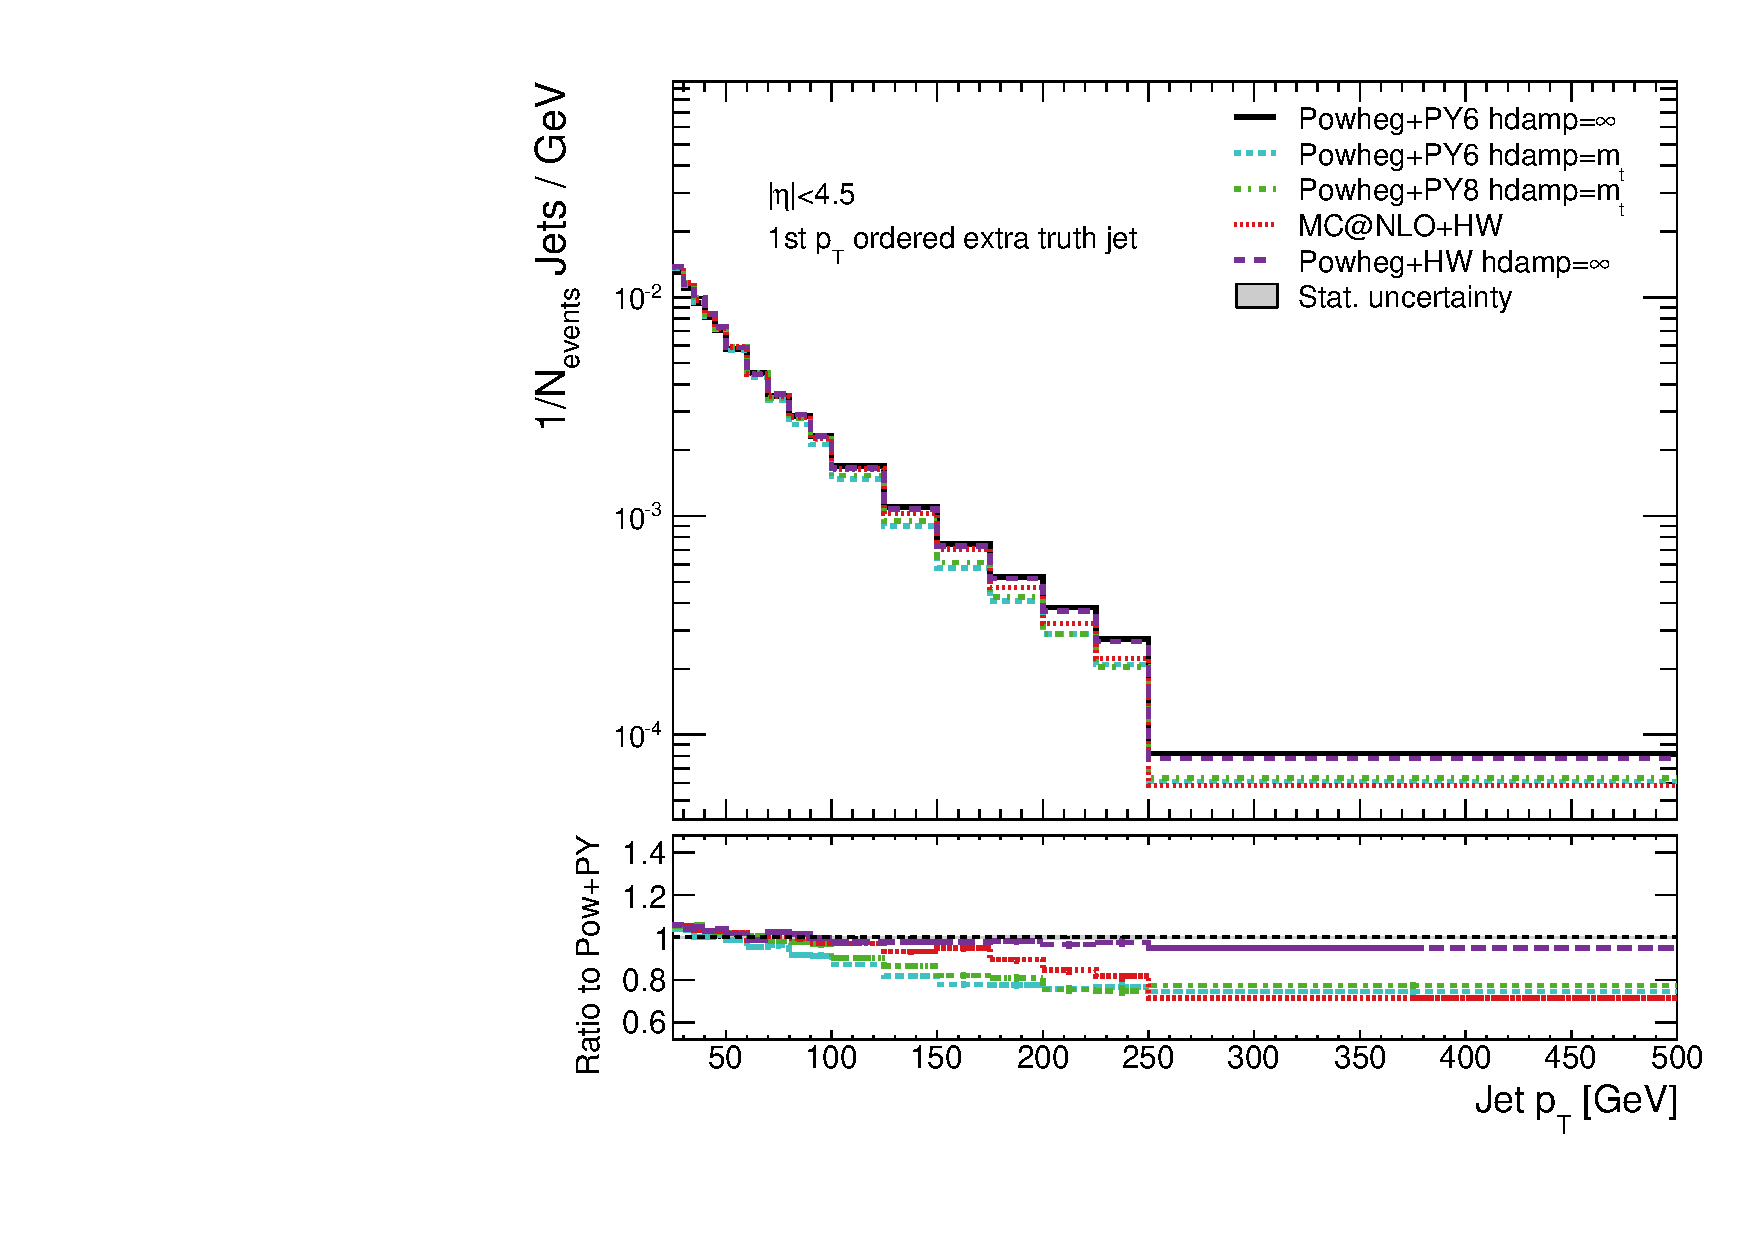
\includegraphics[width=\textwidth]{fig/MCComp/NLO/TruthPtJet0.pdf}
\end{subfigure} ~
\begin{subfigure}[]{0.45\textwidth}
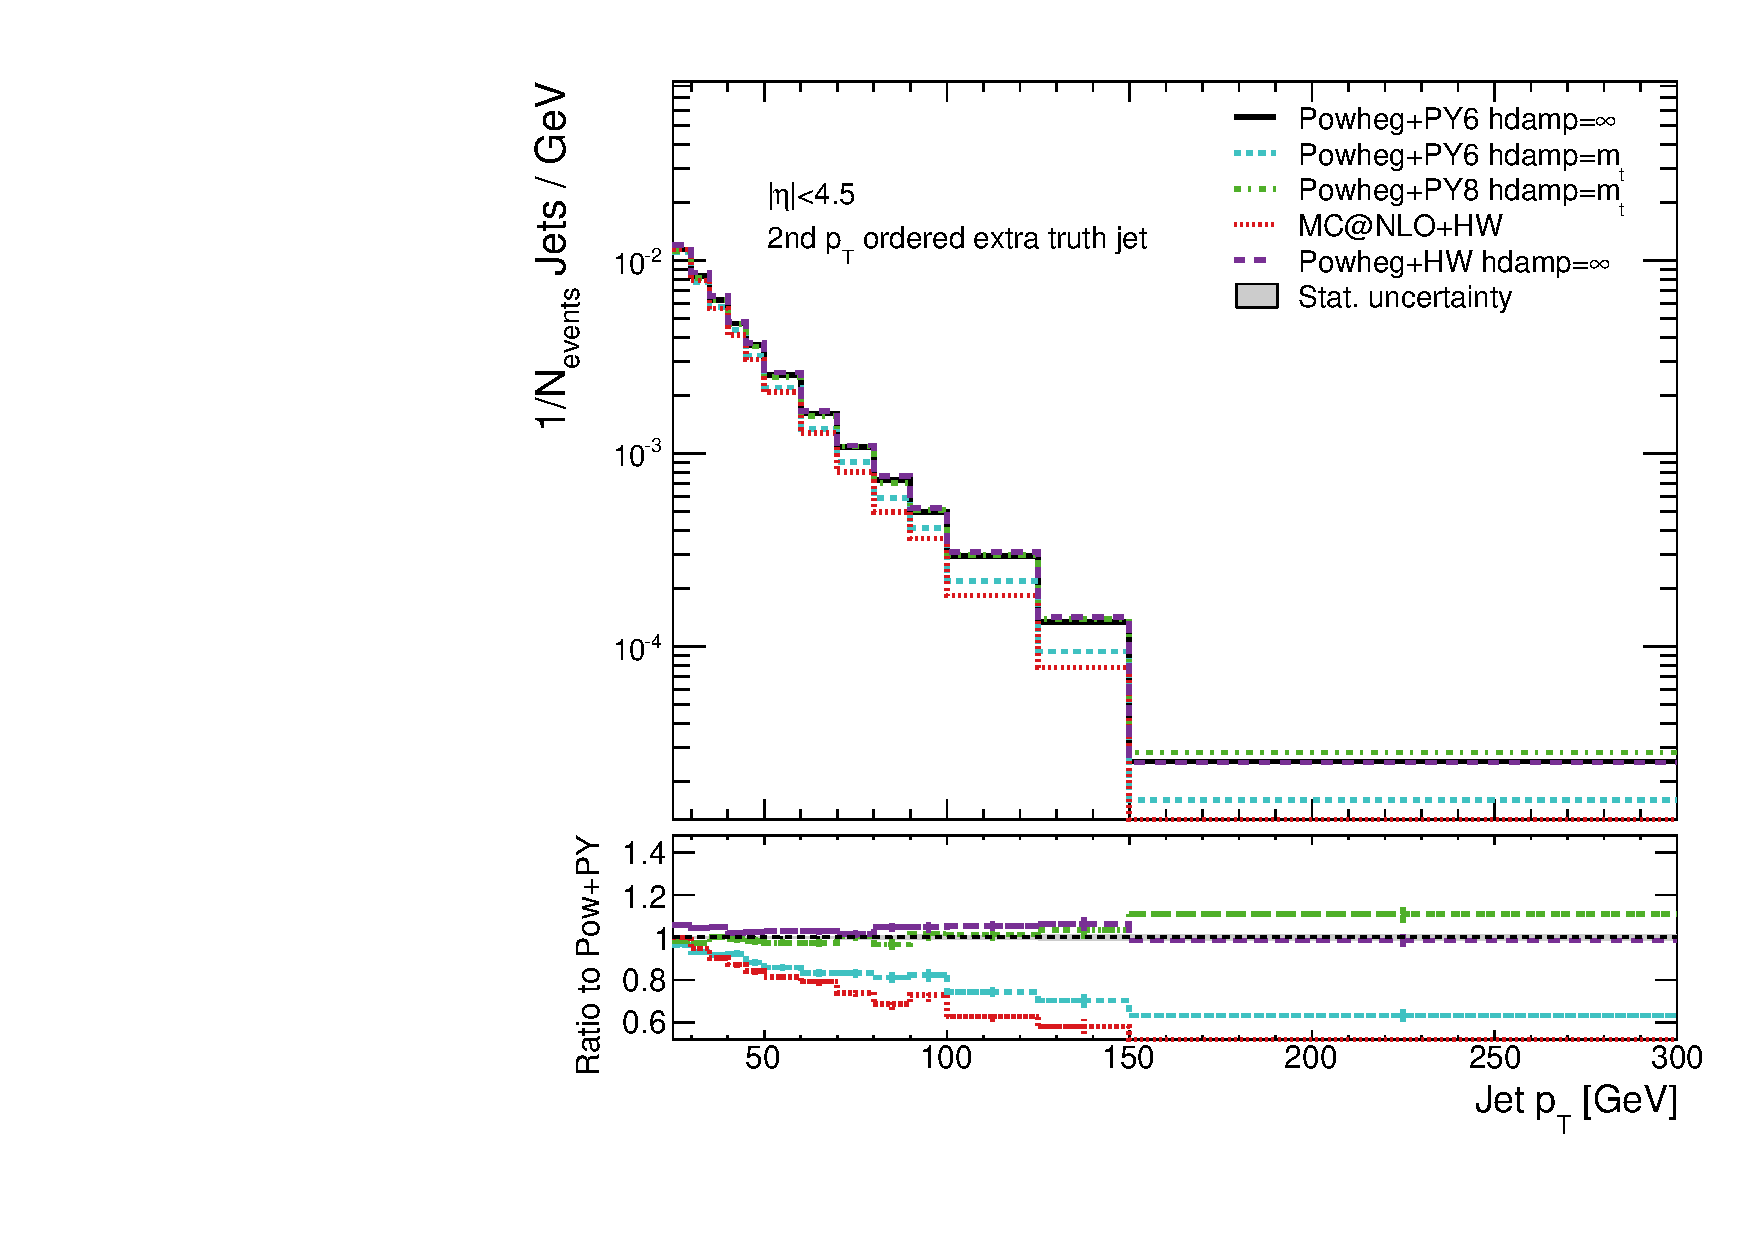
\includegraphics[width=\textwidth]{fig/MCComp/NLO/TruthPtJet1.pdf}
\end{subfigure}
\caption{Comparison of the truth level extra jet multiplicity and $\pt$ distributions in generated $\ttbar$ events with an opposite-sign $e\mu$ pair and at least 2 $b$-jets.  Jets are reconstructed using the anti-$k_t$ algorithm with 
the distance parameter $R=0.4$.
Each simulation is normalized by the number of events passing the truth-level selection.
The ratio plots compare each generator to the predictions of the baseline \textsc{ Powheg+Pythia} sample with the hdamp parameter
set to $\infty$.}
\label{fig:introtjets}
\end{figure}

This thesis presents a measurement of the multiplicity and differential 
cross section for additional (a.k.a. extra) jets produced in 
association with top quark decay products as a function of jet \pT. Events top quarks decaying to the the $e\mu$ final state with at least 2 $b$-tagged jets are used.   Jets are selected from the  $R=0.4$ anti-$k_t$
collection and are calibrated using the final 2012 calibration. These additional jets are ordered 
in transverse momentum and labeled by \textit{rank} $i$, such that $i=1$ represents 
the leading (highest transverse momentum),  $i=2$ the subleading jet, \textit{ etc.}.  The cross sections
\sigmapti\ for $i=1$ through $i=4$ are measured and 
the multiplicity is measured for the number of jets $N_{Jets}=1$ through $N_{Jets}=4$ 
and inclusively for  $N_{Jets}\ge 5$.  Here \sigemubb\ is the fiducial production cross section 
for  events containing a high \pT\ electron, a high \pT\ muon and two tagged \bjet s,
where all four objects are required to pass the fiducial selection:  $\pT>25$~\GeV\ and pseudorapidity $|\eta|<2.5$,
and where the  additional jets in the event are required to have
${p_T}^{i}>25$~\GeV\ and $|\eta^{i}|<4.5$. Thus  $\int$\sigmapti $d{p_T}^{i}$ gives
the fraction of the accepted events that contain at least $i$ jets.

The event selection employed here closely matches that used in the ATLAS 8~\TeV\ cross
section measurement\cite{xsec}. The event rates and background estimates obtained 
are consistent with those obtained for that analysis and result in a sample with a greater than 99\% purity
for the dilepton plus two $b$-jet final state. More than 95\%\ of
the events that pass the reconstruction selection cuts also pass the truth fiducial requirements.

Rather than subtracting $Wt$ events as background, this thesis measures the extra jets from both $Wt$ and \ttbar\ events that pass selection. This choice is motived by the following. At lowest order, the $e\mu+2\ b$-jet final state results from $t\overline t$ production where both the 
$t$ and the $\overline t$  decay leptonically.  
Events where the leptons do not arise from $W$ decay are suppressed by isolation and
transverse momentum cuts on the leptons; they are treated as background and corrected for in the thesis.
The distinction between $t\overline{t}$ and $Wt$ final states cannot be made at NLO in QCD unless the top quark is stable.
Once it decays to $Wb$, the same initial and final state appear in both processes,
\textit{ e.g.} $gg\to W^+W^- b \overline{b}$ appears at LO and NLO via $gg\to  t\overline{t}\to W^+W^- b \overline{b}$ or
at NLO via  $gg\to  Wt\overline{b} \to W^+W^- b \overline{b}$.
Quantum interference must occur and the classification into
``\ttbar'' and ``$Wt$"is not possible. If restrictions are placed on the final state,
 this interference can be restricted and an approximate distinction made. For example,
if a kinematic constraint is applied so both  $W^-\overline{b}$ and  $W^+ b$
have invariant mass equal to the top mass, 
the process is dominated by ``\ttbar'', if  $W^-\overline{b}$ has an invariant mass
far from the top quark mass ``$Wt$" will dominate.
No such kinematic constraint is applied in this thesis, so that any discussion of  ``\ttbar'' 
and ``$Wt$" contributions can only be made in simulation where samples labelled by 
 ``\ttbar'' and ``$Wt$" are used.  In standard ATLAS MC samples, $\sim 3\%$ of the 
$e\mu+2\ b$-jet are assigned to the ``$Wt$" process.  This analysis chooses to treat this
component as signal rather than background as it cannot separate them in a model independent manner. However, if a MC is used to fix the
 ``$Wt$" component, then it can be subtracted from the data and comparisons with ``\ttbar'' MC made. The subtraction will 
introduce (small) additional systematic uncertainties. 


% Additional jets in events passing the selection criteria are selected from the  $R=0.4$ anti-$k_t$
% collection and are calibrated using the final 2012 calibration.  These \pt and \textit{rank} of each 
% jet is encoded into a single bin number. The \textit{rank} of a jet is defined as its \pt order in an event, so that the rank of the leading jet is 1, the rank of the subleading jet is 2, the rank of the subsubleading jet is 3 and so on. 

Reconstructed jets not from the primary vertex are called \textit{unmatched jets} and treated as
background.  Their origin can be studied using simulated samples. In the baseline MC simulation, $\sim 4\%$ of the events 
contain at least one reconstructed calorimeter
jet that cannot be matched to a jet reconstructed from truth particles.  The largest
source of these unmatched jets is pileup interactions.  A second
source is attributable to  detector effects which result in a single truth jet being reconstructed as
two jets in the detector or where  the separation  $\Delta R$ between the reconstructed and truth jet
exceeds the matching cuts.  The rate of unmatched jets is determined as a function of
jet rank and  \pT\ and  is subtracted from the reconstructed distribution before that distribution is
unfolded.

The unfolding procedure used to correct the background-subtracted extra jet \pt~  distributions to the true
spectra takes  reconstruction efficiency and resolution effects
into account.  For events that pass the fiducial requirements at both the truth and the reconstruction level,
a response matrix that maps between truth and reconstruction \pt~ and jet ordering is constructed using simulated data.  The reconstructed spectrum is corrected for migration
of jets with truth \pT\ below the 25~\GeV\ cut but reconstructed \pT\ above it using
a correction factor obtained from simulated data. 
%are incorporated into the response matrix by including extra bins with truth \pT\  below 25~\GeV\ .  
Because the ordered full \pT\  distributions
are corrected with a single unfolding matrix, cases where the relative rank of two reconstructed jets
differs from of their associated truth jets are properly treated in the unfolding.  

%The unfolded distribution is then normalized by the number of events passing the event selection, producing a distribution of the mean number of jets per grand bin per reconstructed event.

The unfolded jet \pT\ spectra provide unbiased measurements of the true transverse momentum distributions of the ordered
jets for events passing the reconstruction-level event selection cuts.   However, they do 
not provide an unbiased measurement of the distributions for events passing the truth fidicial selection.
While most events that pass the reconstruction requirements
also pass the selection cuts at truth level, the inverse is not the case. Only about 25\%\ of the events
passing the truth selection also pass reconstruction.  Furthermore, the event selection efficiency
depends on the kinematics of the top decays;  regions of phase space where the top decay
products have higher \pT\ are more likely to pass the selection criteria.  The resulting bias on
the unfolded distribution is corrected  using bin-by-bin  factors obtained from MC.  
These correction factors typically differ from unity by less than 10\%.


The distribution obtained
after applying this final correction is \sigmapti.  The multiplicity
is obtained by integrating the differential \pT\ distribution separately for each jet rank.



